%----------------------------------------------------------------------------
\label{model}
%----------------------------------------------------------------------------
%----------------------------------------------------------------------------
%bb defines the bounding box for the pdf
%viewport defines the area of the pdf used
%in sidewaysfigure the last entry in bb moves the caption toward/away the pic
%in sidewaysfigure the second entry in bb moves the pic toward/away the caption
%----------------------------------------------------------------------------
\begin{figure}
\scalebox{0.8}[0.8]{
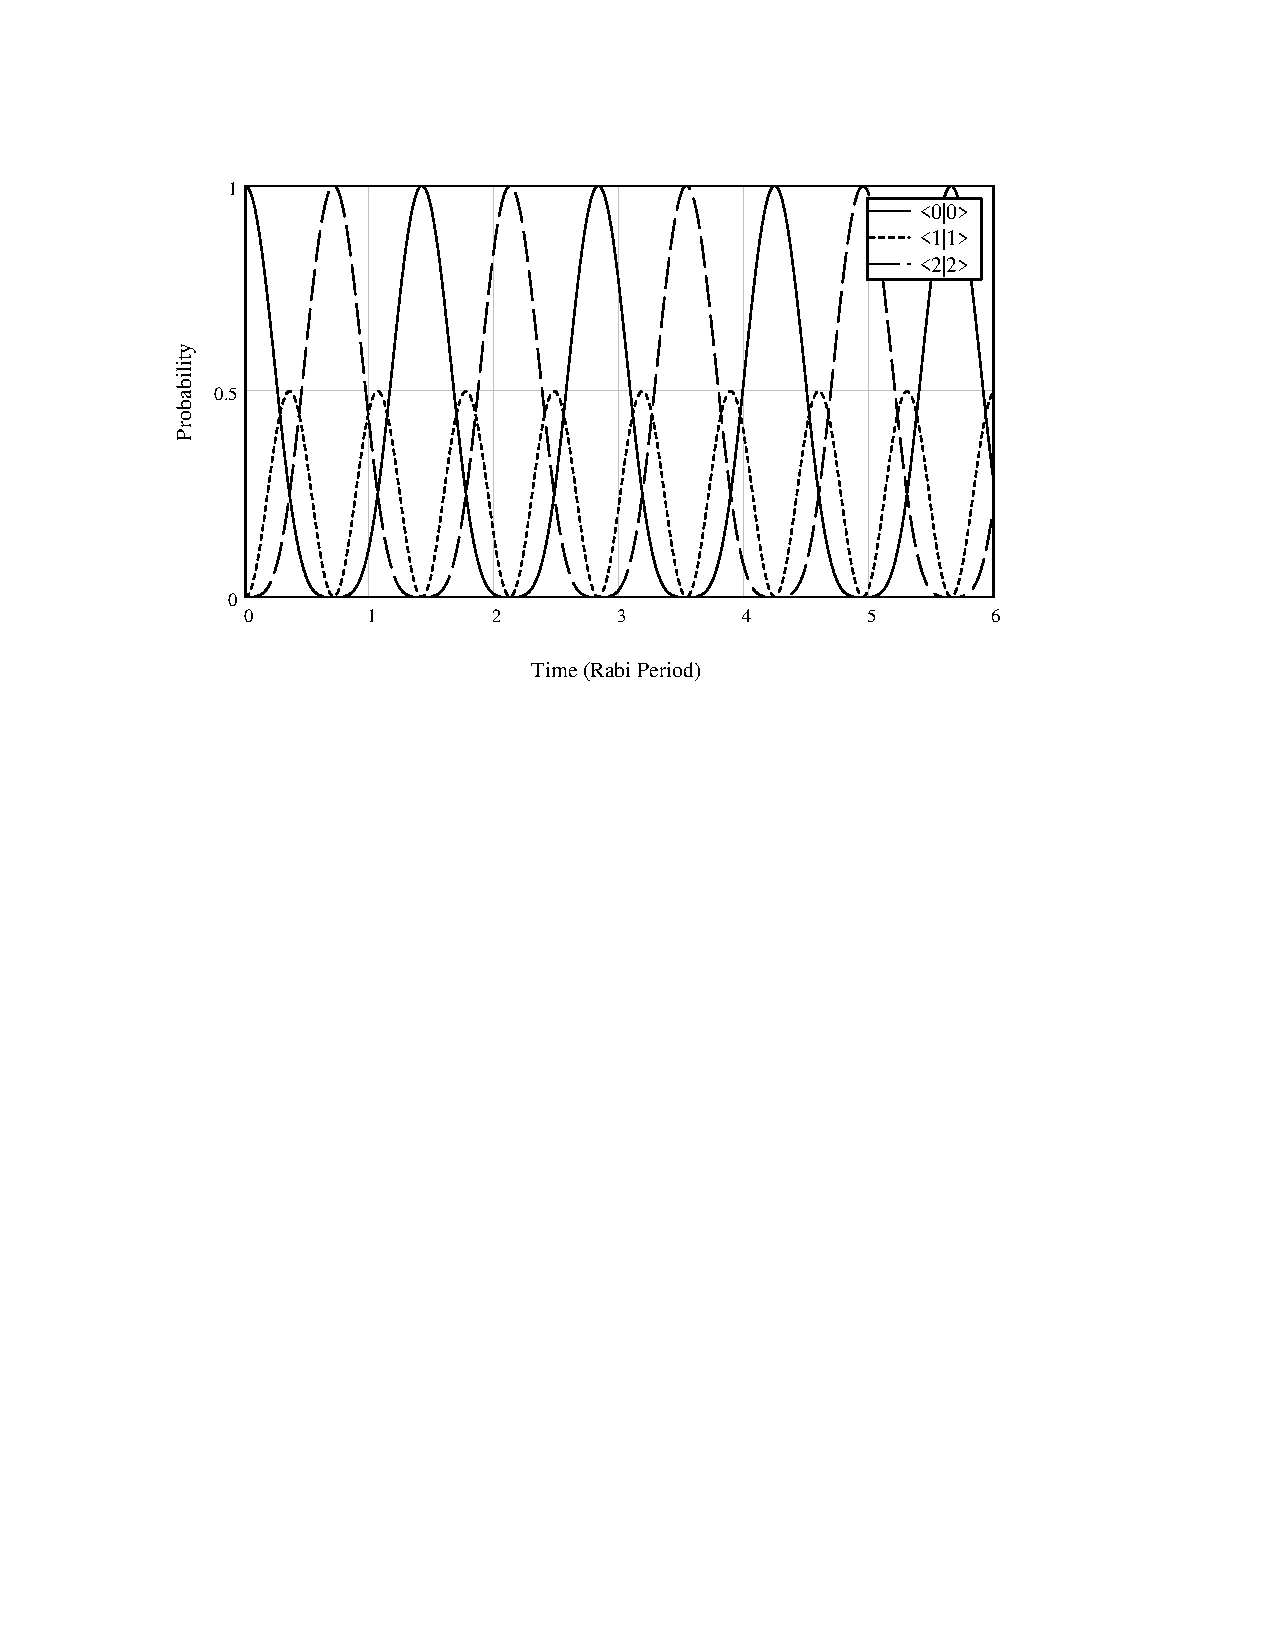
\includegraphics[bb=30 455 489 685]
{clean/clean.pdf}
}
\caption[Collisionless evolution of a three state system]{Collisionless evolution of a three state system. For this (and the following simulations) $\alpha=\beta=1$ and the time scale is the two state Rabi period associated with $\alpha$ (or $\beta$).}
\label{clean}
\end{figure}
%----------------------------------------------------------------------------

%----------------------------------------------------------------------------
%----------------------------------------------------------------------------
%bb defines the bounding box for the pdf
%viewport defines the area of the pdf used
%in sidewaysfigure the last entry in bb moves the caption toward/away the pic
%in sidewaysfigure the second entry in bb moves the pic toward/away the caption
%----------------------------------------------------------------------------
\begin{figure}
\scalebox{0.8}[0.8]{
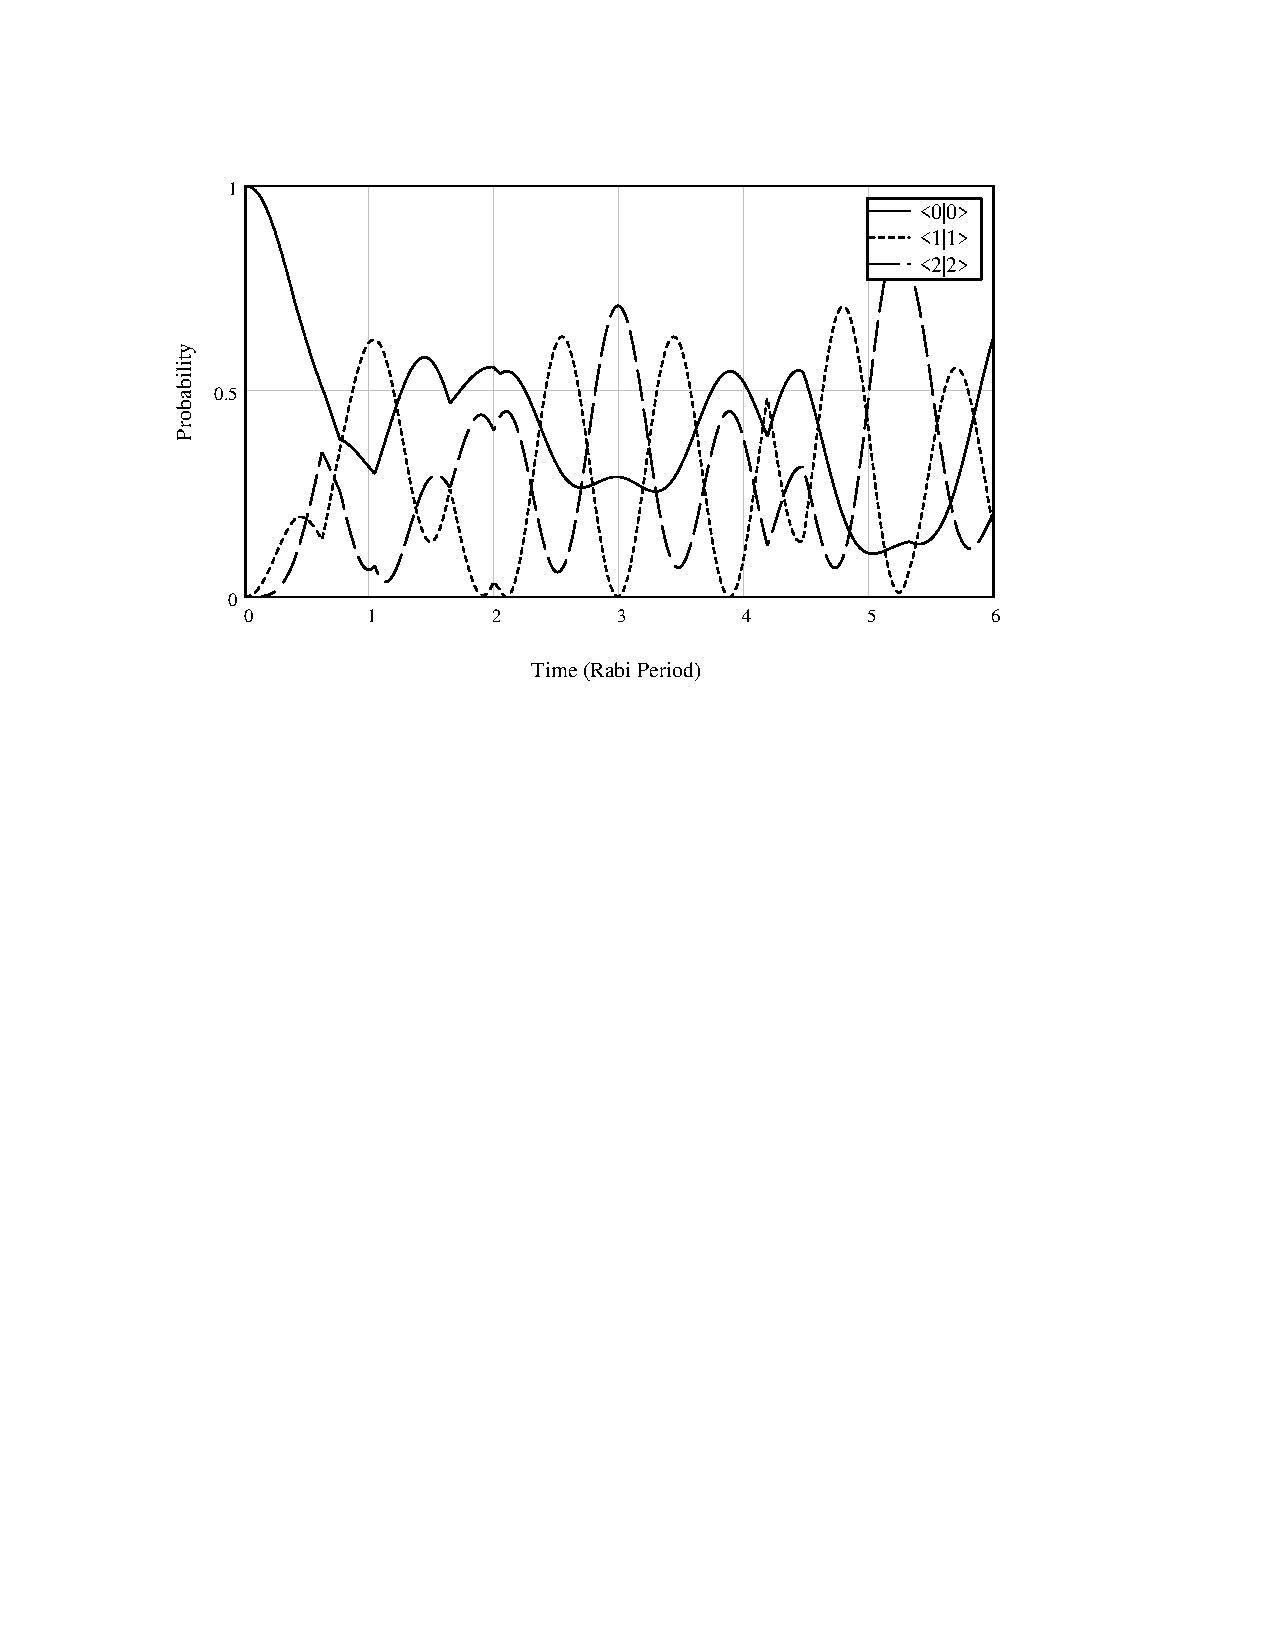
\includegraphics[bb=30 455 489 685]
{coll_1/coll_1.pdf}
}
\caption[Evolution of a three state system with collisions - example 1]{Evolution of a three state system with collisions - example 1. The probability of a collision per Rabi period is 0.5/$\pi$.}
\label{coll_1}
\end{figure}
%----------------------------------------------------------------------------

%----------------------------------------------------------------------------
%----------------------------------------------------------------------------
Reference \cite{Siegman:1986a} describes a model for the collisional effects on the quantum mechanical evolution of an atomic system. The main effect of collisions is to randomize the phase of the expansion coefficients (i.e. the ``c's'' in Equations \ref{expansion} and \ref{se}) as they evolve. (Collisions may also transfer population with relatively low probability in inelastic collisions, but this is ignored in this analysis.) This model is easy to implement in computer code written to solve Equation \ref{se}. As the code solves the equation, it is interrupted randomly. The phase of the expansion coefficients (the expansion coefficients are in general complex) are uniformly randomized on the interval $[0,2\pi)$ while leaving the magnitude intact. Then the numerical integrator picks up where in left off at the interruption, except with the new ``randomized'' expansion coefficients and continues until another ``collision'' (i.e. interruption) takes place. See Figures \ref{clean} through \ref{coll_2} for examples.

The probability of a collision per unit time is arbitrarily selected as $0.5/\pi$ in the examples shown here (there were additional runs at $0.3/\pi$). In Figure \ref{average} we see the result when one million runs are averaged together: the behavior has the appearance of damped oscillations. This behavior seems like it may be described in a cleaner way; if not with an analytic form, then with a differential equation. In the next section we develop a formal candidate.
%----------------------------------------------------------------------------
%----------------------------------------------------------------------------
%bb defines the bounding box for the pdf
%viewport defines the area of the pdf used
%in sidewaysfigure the last entry in bb moves the caption toward/away the pic
%in sidewaysfigure the second entry in bb moves the pic toward/away the caption
%----------------------------------------------------------------------------
\begin{figure}
\scalebox{0.8}[0.8]{
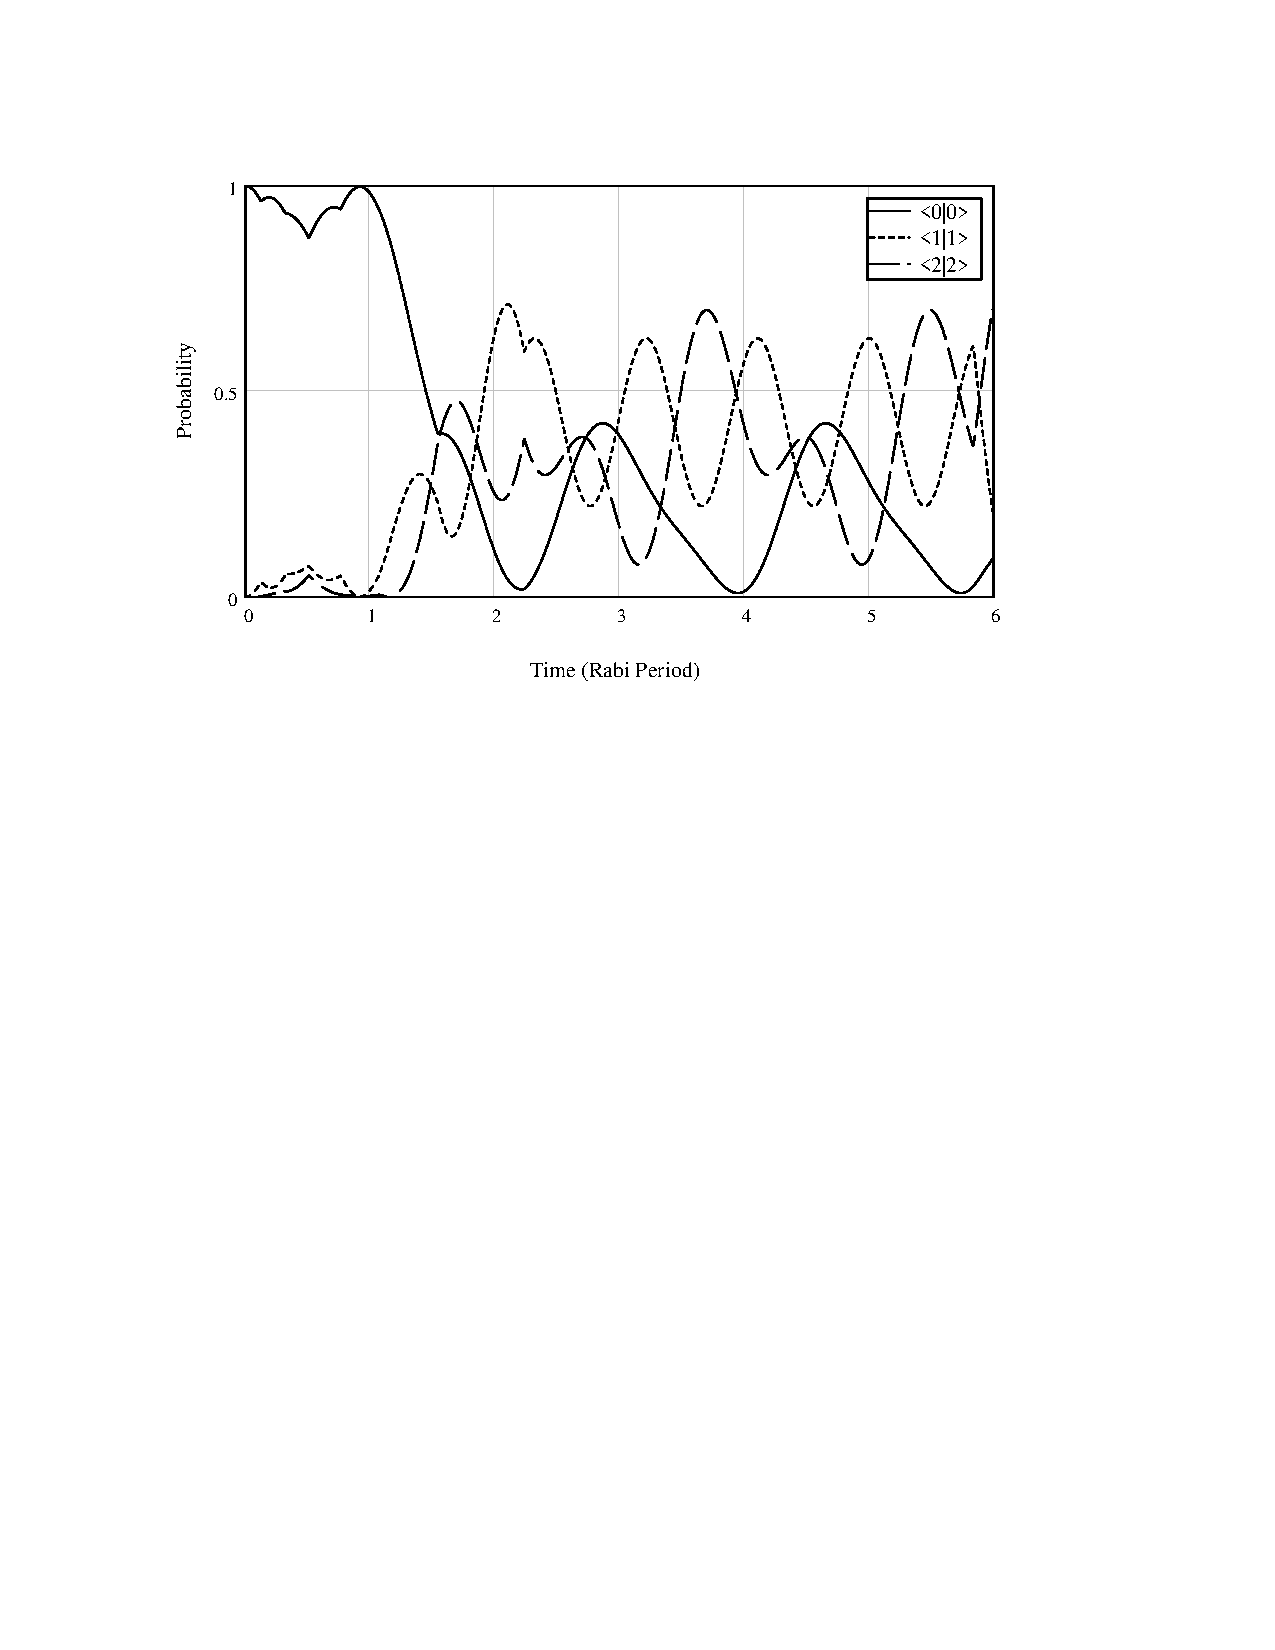
\includegraphics[bb=30 455 489 685]
{coll_2/coll_2.pdf}
}
\caption[Evolution of a three state system with collisions - example 2]{Evolution of a three state system with collisions - example 2. The probability of a collision per Rabi period is 0.5/$\pi$.}
\label{coll_2}
\end{figure}
%----------------------------------------------------------------------------

%----------------------------------------------------------------------------
%----------------------------------------------------------------------------
%----------------------------------------------------------------------------
%----------------------------------------------------------------------------
%----------------------------------------------------------------------------
